\documentclass[]{beamer}
% \usepackage{beamerthemelined}
\usepackage{pstricks}
\usepackage{amsfonts,amssymb,amsmath,amsthm}
\usepackage{graphicx}
\usepackage[]{animate}
\usepackage{wallpaper}
% \setbeamertemplate{navigation symbols}{}
\beamertemplatenavigationsymbolsempty

\usetheme{Boadilla}
\usecolortheme{whale}
\setbeamertemplate{itemize items}[triangle]


\title{}
\author{Paho Lurie-Gregg}
\date{}

\newcommand{\f}[2]{\dfrac{#1}{#2}}
\newcommand{\p}[1]{\left(#1\right)}
\renewcommand{\t}[1]{\text{#1}}
\newcommand{\abs}[1]{\left|#1\right|}

\begin{document}

\begin{frame}
	\frametitle{Generation-  Multilayer Spiral Phase Plate}
	SiO$_2$ is deposited onto a substrate using an electron beam
	\\Since the plate thickness varies with $\phi$, the phase develops the $\phi$ dependence that produces a helical wave front
	\\\centering
	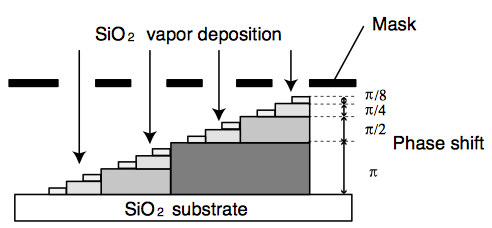
\includegraphics[scale=.4]{MSPP.jpg}
	\\\cite{MSPP}
\end{frame}

\begin{frame}
	\frametitle{Generation - Computer Generated Holography}
	A reference wave and a particular object wave are combined to form an interference pattern.
	\\The interference pattern is then produced as a hologram filament. 
	\\ When a beam propagates through this filament, the first order diffraction beam contains the optical vortex.
\end{frame}

%\begin{frame}

%  \begin{figure}[h]
 %   \centering
  %  \animategraphics[width=\columnwidth, loop]{10}{anim/test-}{01}{39}
 % \end{figure}
%\end{frame}


\end{document}
